\chapter{Analisis}
\label{chap:analisis}

\section{Analisis Kebutuhan Sistem}

\section{Analisis Rancangan Aplikasi}
\subsection{Use Case Diagram}
\begin{figure}[H]
    \centering
    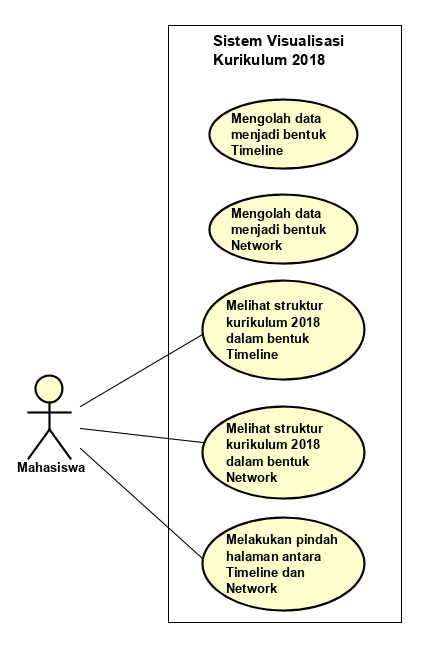
\includegraphics[width=6cm, height=10cm]{Gambar/Use Case.jpg}
    \caption{Use Case Diagram}
    \label{fig:gambarUseCase}
\end{figure}

\begin{itemize}
    \item Sistem akan mengambil data dari \url{https://raw.githubusercontent.com/ftisunpar/data/master/prasyarat.json}.
    \item Sistem mengolah data menjadi bentuk \textit{Timeline}.
    \item Sistem mengolah data menjadi bentuk \textit{Network}.
    \item Mahasiswa melihat struktur kurikulum 2018 dalam bentuk \textit{Timeline}.
    \item Mahasiswa melihat struktur kurikulum 2018 dalam bentuk \textit{Network}.
    \item Mahasiswa dapat melakukan pindah halaman antara halaman \textit{Timeline} dengan halaman \textit{Network}.
\end{itemize}

\subsection{Class Diagram}
\begin{figure}[H]
    \centering
    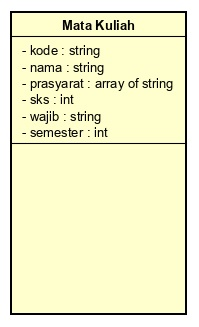
\includegraphics[height=6cm]{Gambar/Class Diagram.jpg}
    \caption{Class Diagram}
    \label{fig:gambarClassDiagram}
\end{figure}

\section{Analisis Hasil Survei}